
\begin{figure}
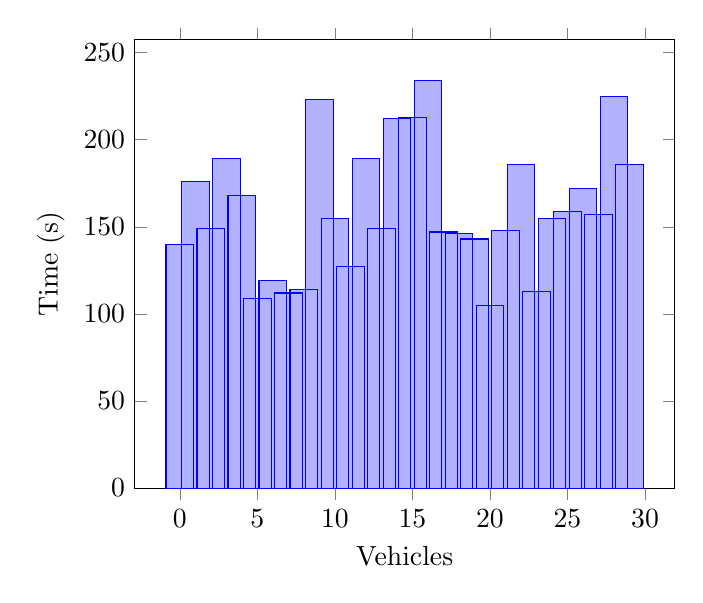
\begin{tikzpicture}
\begin{axis}[
legend style={anchor=west},
xlabel=Vehicles,
ylabel=Time (s),
ymin=0,
ybar,
]
\addplot coordinates {
(0, 140)
(1, 176)
(2, 149)
(3, 189)
(4, 168)
(5, 109)
(6, 119)
(7, 112)
(8, 114)
(9, 223)
(10, 155)
(11, 127)
(12, 189)
(13, 149)
(14, 212)
(15, 213)
(16, 234)
(17, 147)
(18, 146)
(19, 143)
(20, 105)
(21, 148)
(22, 186)
(23, 113)
(24, 155)
(25, 159)
(26, 172)
(27, 157)
(28, 225)
(29, 186)
};

\end{axis}
\end{tikzpicture}
\label{tik:0:21_V, 20_V, 17_N, 15_S, 15_S.-30, 13_N, 13_N.-40, 11_N, 8_N, 7_N, 7_N.-60, 5_N, 4_N, 4_N.-60, 1_N}
\caption{0 percent diving with GSC on route $21_V, 20_V, 17_N, 15_S, 15_S.-30, 13_N, 13_N.-40, 11_N, 8_N, 7_N, 7_N.-60, 5_N, 4_N, 4_N.-60, 1_N$}
\end{figure}
